\subsection{Anti-alias Filter}

Behold the answer in Figure~\ref{fig:2-3}.

\newcommand{\sftt}[1]{
    \begin{subfigure}[b]{0.3\textwidth}
        \includegraphics[width=0.9\textwidth]{../code/2_out/2-3_g#1.png}
        \caption{$\sigma = $#1}
        \label{fig:2-3:#1}
    \end{subfigure}
}

\begin{figure}[h]
\centering

    \begin{subfigure}[b]{0.3\textwidth}
        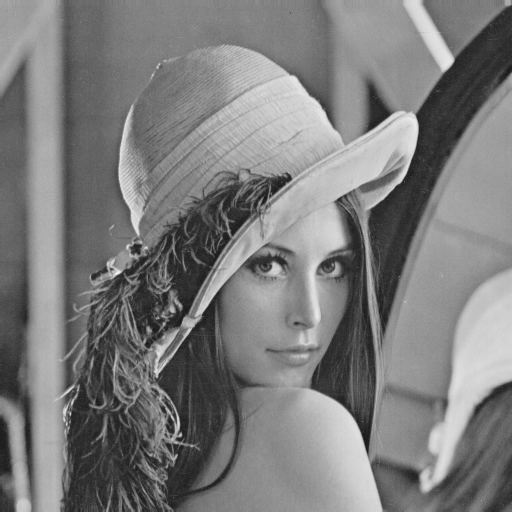
\includegraphics[width=0.9\textwidth]{../code/img/lena.png}
        \caption{Original 512x512 image.}
        \label{fig:2-3:1}
    \end{subfigure}
    \begin{subfigure}[b]{0.3\textwidth}
        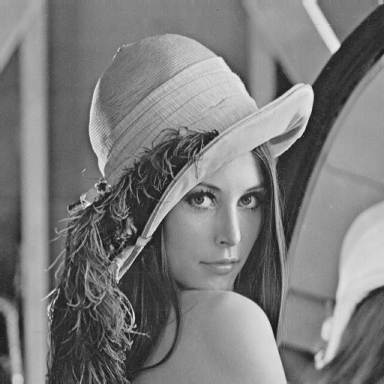
\includegraphics[width=0.9\textwidth]{../code/2_out/2-3_ds.png}
        \caption{3/4ths original size.}
        \label{fig:2-3:1}
    \end{subfigure}

    \sftt{0,5}
    \sftt{1}
    \sftt{2}

    \sftt{4}
    \sftt{8}
    \sftt{16}



\caption{Gaussian filter with varying sigmas applied to aliased image.}
\label{fig:2-3}
\end{figure}

Code used to generate images:
\inputminted[linenos=true]{octave}{../code/2.3.m}
